% Created by tikzDevice version 0.11 on 2018-06-14 22:21:39
% !TEX encoding = UTF-8 Unicode
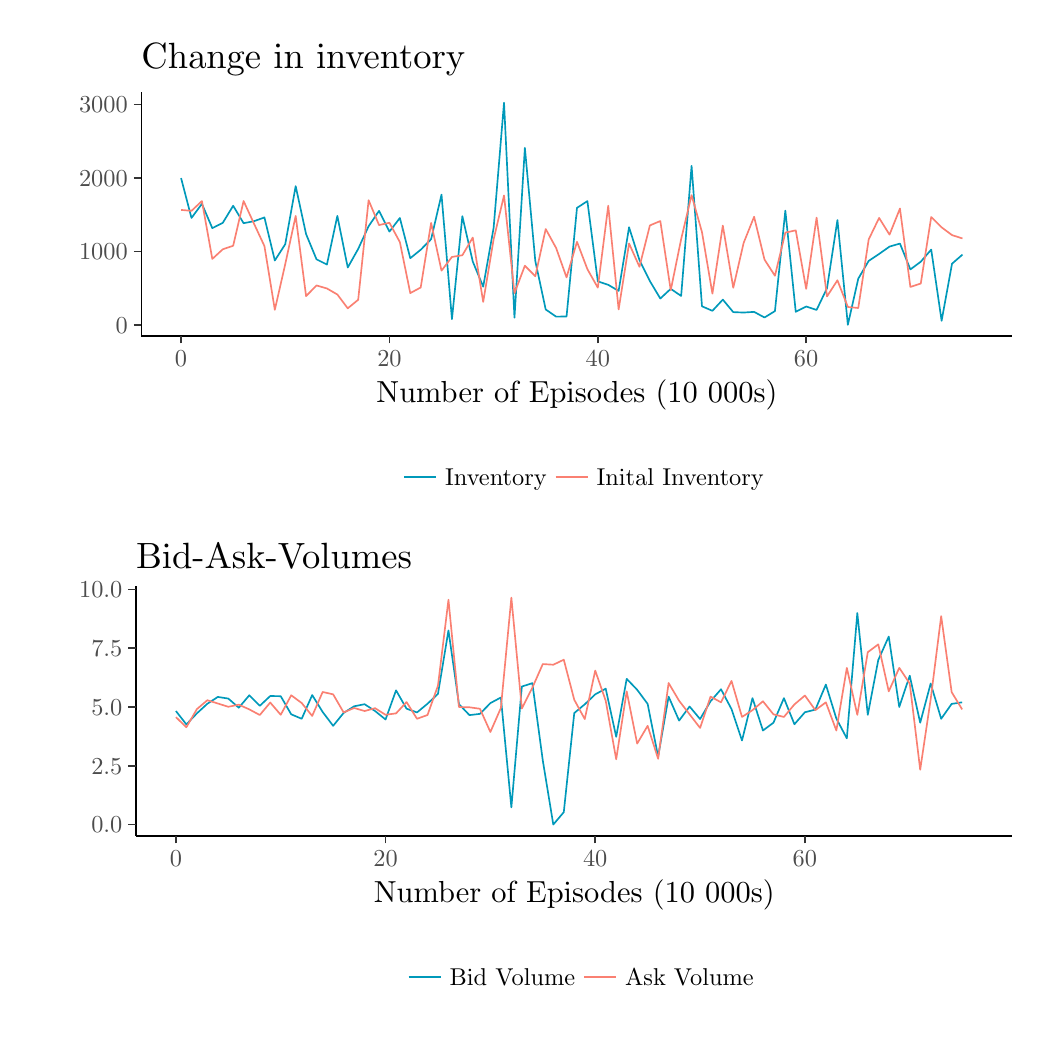
\begin{tikzpicture}[x=1pt,y=1pt]
\definecolor{fillColor}{RGB}{255,255,255}
\path[use as bounding box,fill=fillColor,fill opacity=0.00] (0,0) rectangle (361.35,361.35);
\begin{scope}
\path[clip] (  0.00,180.67) rectangle (361.35,361.35);
\definecolor{drawColor}{RGB}{255,255,255}
\definecolor{fillColor}{RGB}{255,255,255}

\path[draw=drawColor,line width= 0.6pt,line join=round,line cap=round,fill=fillColor] (  0.00,180.67) rectangle (361.35,361.35);
\end{scope}
\begin{scope}
\path[clip] ( 41.12,249.98) rectangle (355.85,338.21);
\definecolor{fillColor}{RGB}{255,255,255}

\path[fill=fillColor] ( 41.12,249.98) rectangle (355.85,338.21);
\definecolor{drawColor}{RGB}{0,153,186}

\path[draw=drawColor,line width= 0.6pt,line join=round] ( 55.43,307.00) --
	( 59.19,292.59) --
	( 62.96,297.69) --
	( 66.72,288.90) --
	( 70.49,290.81) --
	( 74.25,296.99) --
	( 78.02,290.69) --
	( 81.78,291.42) --
	( 85.55,292.77) --
	( 89.31,277.22) --
	( 93.07,283.10) --
	( 96.84,304.09) --
	(100.60,286.75) --
	(104.37,277.64) --
	(108.13,275.76) --
	(111.90,293.33) --
	(115.66,274.68) --
	(119.43,281.40) --
	(123.19,289.58) --
	(126.96,295.15) --
	(130.72,287.66) --
	(134.49,292.57) --
	(138.25,278.04) --
	(142.02,281.10) --
	(145.78,284.91) --
	(149.54,301.02) --
	(153.31,256.03) --
	(157.07,293.22) --
	(160.84,276.81) --
	(164.60,267.76) --
	(168.37,289.03) --
	(172.13,334.20) --
	(175.90,256.55) --
	(179.66,317.93) --
	(183.43,277.04) --
	(187.19,259.52) --
	(190.96,256.92) --
	(194.72,256.99) --
	(198.49,296.23) --
	(202.25,298.67) --
	(206.02,269.66) --
	(209.78,268.43) --
	(213.54,266.22) --
	(217.31,289.21) --
	(221.07,277.37) --
	(224.84,269.76) --
	(228.60,263.48) --
	(232.37,266.98) --
	(236.13,264.40) --
	(239.90,311.40) --
	(243.66,260.67) --
	(247.43,259.03) --
	(251.19,263.08) --
	(254.96,258.56) --
	(258.72,258.41) --
	(262.49,258.65) --
	(266.25,256.62) --
	(270.02,258.93) --
	(273.78,295.23) --
	(277.54,258.68) --
	(281.31,260.59) --
	(285.07,259.36) --
	(288.84,267.21) --
	(292.60,291.83) --
	(296.37,253.99) --
	(300.13,270.65) --
	(303.90,277.07) --
	(307.66,279.58) --
	(311.43,282.24) --
	(315.19,283.34) --
	(318.96,273.99) --
	(322.72,276.78) --
	(326.49,281.16) --
	(330.25,255.43) --
	(334.01,276.06) --
	(337.78,279.33);
\definecolor{drawColor}{RGB}{250,128,114}

\path[draw=drawColor,line width= 0.6pt,line join=round] ( 55.43,295.49) --
	( 59.19,295.15) --
	( 62.96,298.70) --
	( 66.72,277.78) --
	( 70.49,281.26) --
	( 74.25,282.54) --
	( 78.02,298.70) --
	( 81.78,290.53) --
	( 85.55,282.43) --
	( 89.31,259.41) --
	( 93.07,275.90) --
	( 96.84,293.31) --
	(100.60,264.35) --
	(104.37,268.20) --
	(108.13,267.11) --
	(111.90,264.93) --
	(115.66,259.94) --
	(119.43,263.02) --
	(123.19,299.00) --
	(126.96,290.02) --
	(130.72,290.85) --
	(134.49,283.86) --
	(138.25,265.44) --
	(142.02,267.46) --
	(145.78,290.79) --
	(149.54,273.54) --
	(153.31,278.50) --
	(157.07,279.11) --
	(160.84,285.51) --
	(164.60,262.25) --
	(168.37,284.87) --
	(172.13,300.72) --
	(175.90,265.39) --
	(179.66,275.34) --
	(183.43,271.52) --
	(187.19,288.59) --
	(190.96,281.71) --
	(194.72,271.11) --
	(198.49,283.97) --
	(202.25,274.09) --
	(206.02,267.40) --
	(209.78,296.98) --
	(213.54,259.52) --
	(217.31,283.36) --
	(221.07,274.94) --
	(224.84,289.89) --
	(228.60,291.48) --
	(232.37,266.47) --
	(236.13,284.93) --
	(239.90,300.85) --
	(243.66,287.45) --
	(247.43,265.23) --
	(251.19,289.84) --
	(254.96,267.35) --
	(258.72,283.60) --
	(262.49,293.02) --
	(266.25,277.55) --
	(270.02,271.70) --
	(273.78,287.29) --
	(277.54,288.11) --
	(281.31,266.95) --
	(285.07,292.70) --
	(288.84,264.24) --
	(292.60,270.06) --
	(296.37,260.42) --
	(300.13,260.05) --
	(303.90,284.82) --
	(307.66,292.60) --
	(311.43,286.55) --
	(315.19,296.00) --
	(318.96,267.67) --
	(322.72,268.89) --
	(326.49,292.92) --
	(330.25,289.20) --
	(334.01,286.39) --
	(337.78,285.19);
\end{scope}
\begin{scope}
\path[clip] (  0.00,  0.00) rectangle (361.35,361.35);
\definecolor{drawColor}{RGB}{0,0,0}

\path[draw=drawColor,line width= 0.6pt,line join=round] ( 41.12,249.98) --
	( 41.12,338.21);
\end{scope}
\begin{scope}
\path[clip] (  0.00,  0.00) rectangle (361.35,361.35);
\definecolor{drawColor}{gray}{0.30}

\node[text=drawColor,anchor=base east,inner sep=0pt, outer sep=0pt, scale=  0.88] at ( 36.17,250.89) {0};

\node[text=drawColor,anchor=base east,inner sep=0pt, outer sep=0pt, scale=  0.88] at ( 36.17,277.44) {1000};

\node[text=drawColor,anchor=base east,inner sep=0pt, outer sep=0pt, scale=  0.88] at ( 36.17,303.98) {2000};

\node[text=drawColor,anchor=base east,inner sep=0pt, outer sep=0pt, scale=  0.88] at ( 36.17,330.53) {3000};
\end{scope}
\begin{scope}
\path[clip] (  0.00,  0.00) rectangle (361.35,361.35);
\definecolor{drawColor}{gray}{0.20}

\path[draw=drawColor,line width= 0.6pt,line join=round] ( 38.37,253.92) --
	( 41.12,253.92);

\path[draw=drawColor,line width= 0.6pt,line join=round] ( 38.37,280.47) --
	( 41.12,280.47);

\path[draw=drawColor,line width= 0.6pt,line join=round] ( 38.37,307.01) --
	( 41.12,307.01);

\path[draw=drawColor,line width= 0.6pt,line join=round] ( 38.37,333.56) --
	( 41.12,333.56);
\end{scope}
\begin{scope}
\path[clip] (  0.00,  0.00) rectangle (361.35,361.35);
\definecolor{drawColor}{RGB}{0,0,0}

\path[draw=drawColor,line width= 0.6pt,line join=round] ( 41.12,249.98) --
	(355.85,249.98);
\end{scope}
\begin{scope}
\path[clip] (  0.00,  0.00) rectangle (361.35,361.35);
\definecolor{drawColor}{gray}{0.20}

\path[draw=drawColor,line width= 0.6pt,line join=round] ( 55.43,247.23) --
	( 55.43,249.98);

\path[draw=drawColor,line width= 0.6pt,line join=round] (130.72,247.23) --
	(130.72,249.98);

\path[draw=drawColor,line width= 0.6pt,line join=round] (206.02,247.23) --
	(206.02,249.98);

\path[draw=drawColor,line width= 0.6pt,line join=round] (281.31,247.23) --
	(281.31,249.98);
\end{scope}
\begin{scope}
\path[clip] (  0.00,  0.00) rectangle (361.35,361.35);
\definecolor{drawColor}{gray}{0.30}

\node[text=drawColor,anchor=base,inner sep=0pt, outer sep=0pt, scale=  0.88] at ( 55.43,238.97) {0};

\node[text=drawColor,anchor=base,inner sep=0pt, outer sep=0pt, scale=  0.88] at (130.72,238.97) {20};

\node[text=drawColor,anchor=base,inner sep=0pt, outer sep=0pt, scale=  0.88] at (206.02,238.97) {40};

\node[text=drawColor,anchor=base,inner sep=0pt, outer sep=0pt, scale=  0.88] at (281.31,238.97) {60};
\end{scope}
\begin{scope}
\path[clip] (  0.00,  0.00) rectangle (361.35,361.35);
\definecolor{drawColor}{RGB}{0,0,0}

\node[text=drawColor,anchor=base,inner sep=0pt, outer sep=0pt, scale=  1.10] at (198.49,225.89) {Number of Episodes (10 000s)};
\end{scope}
\begin{scope}
\path[clip] (  0.00,  0.00) rectangle (361.35,361.35);
\definecolor{fillColor}{RGB}{255,255,255}

\path[fill=fillColor] (125.29,186.17) rectangle (271.68,212.01);
\end{scope}
\begin{scope}
\path[clip] (  0.00,  0.00) rectangle (361.35,361.35);
\definecolor{drawColor}{RGB}{0,153,186}

\path[draw=drawColor,line width= 0.6pt,line join=round] (136.04,199.09) -- (147.60,199.09);
\end{scope}
\begin{scope}
\path[clip] (  0.00,  0.00) rectangle (361.35,361.35);
\definecolor{drawColor}{RGB}{250,128,114}

\path[draw=drawColor,line width= 0.6pt,line join=round] (190.79,199.09) -- (202.35,199.09);
\end{scope}
\begin{scope}
\path[clip] (  0.00,  0.00) rectangle (361.35,361.35);
\definecolor{drawColor}{RGB}{0,0,0}

\node[text=drawColor,anchor=base west,inner sep=0pt, outer sep=0pt, scale=  0.88] at (150.85,196.06) {Inventory};
\end{scope}
\begin{scope}
\path[clip] (  0.00,  0.00) rectangle (361.35,361.35);
\definecolor{drawColor}{RGB}{0,0,0}

\node[text=drawColor,anchor=base west,inner sep=0pt, outer sep=0pt, scale=  0.88] at (205.60,196.06) {Inital Inventory};
\end{scope}
\begin{scope}
\path[clip] (  0.00,  0.00) rectangle (361.35,361.35);
\definecolor{drawColor}{RGB}{0,0,0}

\node[text=drawColor,anchor=base west,inner sep=0pt, outer sep=0pt, scale=  1.32] at ( 41.12,346.76) {Change in inventory};
\end{scope}
\begin{scope}
\path[clip] (  0.00,  0.00) rectangle (361.35,180.67);
\definecolor{drawColor}{RGB}{255,255,255}
\definecolor{fillColor}{RGB}{255,255,255}

\path[draw=drawColor,line width= 0.6pt,line join=round,line cap=round,fill=fillColor] (  0.00, -0.00) rectangle (361.35,180.67);
\end{scope}
\begin{scope}
\path[clip] ( 39.17, 69.30) rectangle (355.85,159.48);
\definecolor{fillColor}{RGB}{255,255,255}

\path[fill=fillColor] ( 39.17, 69.30) rectangle (355.85,159.48);
\definecolor{drawColor}{RGB}{0,153,186}

\path[draw=drawColor,line width= 0.6pt,line join=round] ( 53.56,114.42) --
	( 57.35,109.58) --
	( 61.14,113.57) --
	( 64.93,117.05) --
	( 68.71,119.51) --
	( 72.50,118.92) --
	( 76.29,115.61) --
	( 80.08,120.11) --
	( 83.87,116.29) --
	( 87.65,119.85) --
	( 91.44,119.77) --
	( 95.23,113.23) --
	( 99.02,111.62) --
	(102.81,120.19) --
	(106.59,114.08) --
	(110.38,109.07) --
	(114.17,113.74) --
	(117.96,116.12) --
	(121.75,116.88) --
	(125.53,114.42) --
	(129.32,111.36) --
	(133.11,121.89) --
	(136.90,115.27) --
	(140.69,113.91) --
	(144.48,117.05) --
	(148.26,120.62) --
	(152.05,143.55) --
	(155.84,116.92) --
	(159.63,112.94) --
	(163.42,113.39) --
	(167.20,117.28) --
	(170.99,119.31) --
	(174.78, 79.61) --
	(178.57,123.26) --
	(182.36,124.49) --
	(186.14, 96.53) --
	(189.93, 73.40) --
	(193.72, 77.87) --
	(197.51,113.69) --
	(201.30,116.84) --
	(205.08,120.44) --
	(208.87,122.50) --
	(212.66,105.11) --
	(216.45,126.05) --
	(220.24,122.09) --
	(224.02,117.00) --
	(227.81, 97.93) --
	(231.60,119.64) --
	(235.39,110.96) --
	(239.18,116.05) --
	(242.97,111.52) --
	(246.75,117.94) --
	(250.54,122.28) --
	(254.33,115.11) --
	(258.12,103.78) --
	(261.91,119.07) --
	(265.69,107.37) --
	(269.48,110.20) --
	(273.27,119.07) --
	(277.06,109.64) --
	(280.85,113.98) --
	(284.63,114.92) --
	(288.42,123.98) --
	(292.21,111.71) --
	(296.00,104.54) --
	(299.79,149.83) --
	(303.57,113.03) --
	(307.36,132.85) --
	(311.15,141.34) --
	(314.94,115.86) --
	(318.73,127.19) --
	(322.51,110.20) --
	(326.30,124.36) --
	(330.09,111.62) --
	(333.88,117.00) --
	(337.67,117.56);
\definecolor{drawColor}{RGB}{250,128,114}

\path[draw=drawColor,line width= 0.6pt,line join=round] ( 53.56,112.21) --
	( 57.35,108.56) --
	( 61.14,115.10) --
	( 64.93,118.33) --
	( 68.71,117.14) --
	( 72.50,115.95) --
	( 76.29,116.71) --
	( 80.08,115.01) --
	( 83.87,112.98) --
	( 87.65,117.48) --
	( 91.44,113.06) --
	( 95.23,120.11) --
	( 99.02,117.31) --
	(102.81,112.64) --
	(106.59,121.30) --
	(110.38,120.45) --
	(114.17,113.91) --
	(117.96,115.52) --
	(121.75,114.42) --
	(125.53,115.44) --
	(129.32,113.06) --
	(133.11,113.57) --
	(136.90,117.65) --
	(140.69,111.62) --
	(144.48,112.98) --
	(148.26,123.59) --
	(152.05,154.61) --
	(155.84,115.86) --
	(159.63,115.77) --
	(163.42,115.24) --
	(167.20,106.84) --
	(170.99,115.51) --
	(174.78,155.38) --
	(178.57,115.32) --
	(182.36,122.85) --
	(186.14,131.39) --
	(189.93,131.15) --
	(193.72,132.96) --
	(197.51,118.48) --
	(201.30,111.51) --
	(205.08,129.04) --
	(208.87,118.15) --
	(212.66, 96.99) --
	(216.45,121.52) --
	(220.24,102.65) --
	(224.02,109.07) --
	(227.81, 97.18) --
	(231.60,124.54) --
	(235.39,118.13) --
	(239.18,113.22) --
	(242.97,108.31) --
	(246.75,119.64) --
	(250.54,117.56) --
	(254.33,125.30) --
	(258.12,112.28) --
	(261.91,114.73) --
	(265.69,117.94) --
	(269.48,113.22) --
	(273.27,112.28) --
	(277.06,116.81) --
	(280.85,120.01) --
	(284.63,114.73) --
	(288.42,117.56) --
	(292.21,107.37) --
	(296.00,130.02) --
	(299.79,113.03) --
	(303.57,135.68) --
	(307.36,138.51) --
	(311.15,121.52) --
	(314.94,130.02) --
	(318.73,124.36) --
	(322.51, 93.22) --
	(326.30,118.69) --
	(330.09,148.70) --
	(333.88,121.24) --
	(337.67,115.01);
\end{scope}
\begin{scope}
\path[clip] (  0.00,  0.00) rectangle (361.35,361.35);
\definecolor{drawColor}{RGB}{0,0,0}

\path[draw=drawColor,line width= 0.6pt,line join=round] ( 39.17, 69.30) --
	( 39.17,159.48);
\end{scope}
\begin{scope}
\path[clip] (  0.00,  0.00) rectangle (361.35,361.35);
\definecolor{drawColor}{gray}{0.30}

\node[text=drawColor,anchor=base east,inner sep=0pt, outer sep=0pt, scale=  0.88] at ( 34.22, 70.37) {0.0};

\node[text=drawColor,anchor=base east,inner sep=0pt, outer sep=0pt, scale=  0.88] at ( 34.22, 91.60) {2.5};

\node[text=drawColor,anchor=base east,inner sep=0pt, outer sep=0pt, scale=  0.88] at ( 34.22,112.83) {5.0};

\node[text=drawColor,anchor=base east,inner sep=0pt, outer sep=0pt, scale=  0.88] at ( 34.22,134.06) {7.5};

\node[text=drawColor,anchor=base east,inner sep=0pt, outer sep=0pt, scale=  0.88] at ( 34.22,155.29) {10.0};
\end{scope}
\begin{scope}
\path[clip] (  0.00,  0.00) rectangle (361.35,361.35);
\definecolor{drawColor}{gray}{0.20}

\path[draw=drawColor,line width= 0.6pt,line join=round] ( 36.42, 73.40) --
	( 39.17, 73.40);

\path[draw=drawColor,line width= 0.6pt,line join=round] ( 36.42, 94.63) --
	( 39.17, 94.63);

\path[draw=drawColor,line width= 0.6pt,line join=round] ( 36.42,115.86) --
	( 39.17,115.86);

\path[draw=drawColor,line width= 0.6pt,line join=round] ( 36.42,137.09) --
	( 39.17,137.09);

\path[draw=drawColor,line width= 0.6pt,line join=round] ( 36.42,158.32) --
	( 39.17,158.32);
\end{scope}
\begin{scope}
\path[clip] (  0.00,  0.00) rectangle (361.35,361.35);
\definecolor{drawColor}{RGB}{0,0,0}

\path[draw=drawColor,line width= 0.6pt,line join=round] ( 39.17, 69.30) --
	(355.85, 69.30);
\end{scope}
\begin{scope}
\path[clip] (  0.00,  0.00) rectangle (361.35,361.35);
\definecolor{drawColor}{gray}{0.20}

\path[draw=drawColor,line width= 0.6pt,line join=round] ( 53.56, 66.55) --
	( 53.56, 69.30);

\path[draw=drawColor,line width= 0.6pt,line join=round] (129.32, 66.55) --
	(129.32, 69.30);

\path[draw=drawColor,line width= 0.6pt,line join=round] (205.08, 66.55) --
	(205.08, 69.30);

\path[draw=drawColor,line width= 0.6pt,line join=round] (280.85, 66.55) --
	(280.85, 69.30);
\end{scope}
\begin{scope}
\path[clip] (  0.00,  0.00) rectangle (361.35,361.35);
\definecolor{drawColor}{gray}{0.30}

\node[text=drawColor,anchor=base,inner sep=0pt, outer sep=0pt, scale=  0.88] at ( 53.56, 58.29) {0};

\node[text=drawColor,anchor=base,inner sep=0pt, outer sep=0pt, scale=  0.88] at (129.32, 58.29) {20};

\node[text=drawColor,anchor=base,inner sep=0pt, outer sep=0pt, scale=  0.88] at (205.08, 58.29) {40};

\node[text=drawColor,anchor=base,inner sep=0pt, outer sep=0pt, scale=  0.88] at (280.85, 58.29) {60};
\end{scope}
\begin{scope}
\path[clip] (  0.00,  0.00) rectangle (361.35,361.35);
\definecolor{drawColor}{RGB}{0,0,0}

\node[text=drawColor,anchor=base,inner sep=0pt, outer sep=0pt, scale=  1.10] at (197.51, 45.22) {Number of Episodes (10 000s)};
\end{scope}
\begin{scope}
\path[clip] (  0.00,  0.00) rectangle (361.35,361.35);
\definecolor{fillColor}{RGB}{255,255,255}

\path[fill=fillColor] (126.94,  5.50) rectangle (268.08, 31.34);
\end{scope}
\begin{scope}
\path[clip] (  0.00,  0.00) rectangle (361.35,361.35);
\definecolor{drawColor}{RGB}{0,153,186}

\path[draw=drawColor,line width= 0.6pt,line join=round] (137.69, 18.42) -- (149.25, 18.42);
\end{scope}
\begin{scope}
\path[clip] (  0.00,  0.00) rectangle (361.35,361.35);
\definecolor{drawColor}{RGB}{250,128,114}

\path[draw=drawColor,line width= 0.6pt,line join=round] (201.09, 18.42) -- (212.65, 18.42);
\end{scope}
\begin{scope}
\path[clip] (  0.00,  0.00) rectangle (361.35,361.35);
\definecolor{drawColor}{RGB}{0,0,0}

\node[text=drawColor,anchor=base west,inner sep=0pt, outer sep=0pt, scale=  0.88] at (152.50, 15.39) {Bid Volume};
\end{scope}
\begin{scope}
\path[clip] (  0.00,  0.00) rectangle (361.35,361.35);
\definecolor{drawColor}{RGB}{0,0,0}

\node[text=drawColor,anchor=base west,inner sep=0pt, outer sep=0pt, scale=  0.88] at (215.90, 15.39) {Ask Volume};
\end{scope}
\begin{scope}
\path[clip] (  0.00,  0.00) rectangle (361.35,361.35);
\definecolor{drawColor}{RGB}{0,0,0}

\node[text=drawColor,anchor=base west,inner sep=0pt, outer sep=0pt, scale=  1.32] at ( 39.17,166.08) {Bid-Ask-Volumes};
\end{scope}
\end{tikzpicture}
